\documentclass[conference]{IEEEtran}

\usepackage{cite}
\usepackage{amsmath,amssymb,amsfonts}
\usepackage{algorithmic}
\usepackage{algorithm}
\usepackage{graphicx}
\usepackage{textcomp}
\usepackage{booktabs}
\usepackage{multirow}
\usepackage{xcolor}
\usepackage{hyperref}
\usepackage{subcaption}

\graphicspath{{figures/}}

\begin{document}

\title{GNN-DQN Hybrid Spectrum Management for 5G NR--Radar Coexistence in Shared Mid-Band Spectrum}

\author{
\IEEEauthorblockN{Fahmida Afrin}
\IEEEauthorblockA{Department of Electrical and Computer Engineering\\
\textit{University}}
}

\maketitle

% ===========================================================================
% ABSTRACT
% ===========================================================================
\begin{abstract}
Mid-band spectrum sharing between 5G New Radio (NR) and pulsed radar systems presents a critical challenge for next-generation wireless networks. Existing schedulers---Round Robin, Proportional Fair, and Best-CQI---are agnostic to radar interference patterns, leading to degraded throughput, elevated block error rates (BLER), and excessive HARQ retransmissions in coexistence scenarios. We propose a hybrid Graph Neural Network--Deep Q-Network (GNN-DQN) framework for intelligent Physical Resource Block (PRB) allocation that jointly optimizes spectral efficiency, radar interference avoidance, and user fairness. The GNN component models inter-PRB relationships and spatial interference structure through a graph representation of the resource grid, while the DQN component learns adaptive allocation policies via reinforcement learning with prioritized experience replay. We evaluate the proposed approach against three standard schedulers using a high-fidelity MATLAB-based 5G NR TDD simulation with waveform-level Linear Frequency Modulated (LFM) radar injection at 3.5\,GHz. Experimental results across varying radar duty cycles (1--20\%), pulse parameters, and network configurations demonstrate that the hybrid GNN-DQN achieves up to 30\% higher throughput, 95\% radar band protection, and 40\% faster interference evacuation compared to the best conventional scheduler, while maintaining Jain's fairness index above 0.85.
\end{abstract}

\begin{IEEEkeywords}
5G NR, radar coexistence, spectrum sharing, graph neural network, deep reinforcement learning, resource allocation, O-RAN
\end{IEEEkeywords}

% ===========================================================================
% 1. INTRODUCTION
% ===========================================================================
\section{Introduction}

The proliferation of 5G New Radio (NR) services in the 3.1--3.55\,GHz Citizens Broadband Radio Service (CBRS) and 3.55--3.7\,GHz mid-band spectrum has intensified the coexistence challenge with incumbent pulsed radar systems \cite{labib2017coexistence, zheng2019spectrum}. Federal radar systems operating in these bands---including shipborne and airborne surveillance radars---transmit high-power Linear Frequency Modulated (LFM) pulses that can severely degrade 5G NR physical layer performance, corrupting OFDM symbol reception, reducing Signal-to-Interference-plus-Noise Ratio (SINR), and triggering excessive Hybrid Automatic Repeat Request (HARQ) retransmissions \cite{sharma2020radar5g}.

Current 3GPP-compliant schedulers allocate Physical Resource Blocks (PRBs) without awareness of radar interference patterns. Round Robin distributes resources equally but wastes capacity on radar-affected PRBs. Proportional Fair balances throughput and fairness but cannot anticipate pulsed interference. Best-CQI maximizes instantaneous channel quality but concentrates resources on few users while still allocating radar-corrupted PRBs \cite{3gpp_ts38214}.

Recent advances in Graph Neural Networks (GNNs) for wireless resource management \cite{shen2021graph_resource, he2021gnn_wireless} and Deep Reinforcement Learning (DRL) for spectrum access \cite{lee2020drl_resource, nasir2021gnn_resource} motivate a learning-based approach. However, existing works largely address either static interference scenarios or lack the structural modeling needed to capture PRB-level radar overlap patterns.

\subsection{Contributions}

This paper makes the following contributions:

\begin{enumerate}
    \item \textbf{Graph-based PRB representation:} We model the 5G NR resource grid as a graph where nodes represent PRBs with features derived from per-UE Channel Quality Indicators (CQI), radar activity flags, and BLER measurements. Edges encode frequency adjacency and shared-UE allocation relationships.

    \item \textbf{Hybrid GNN-DQN architecture:} We propose a novel architecture combining a GNN feature extractor (GCN/GAT/GraphSAGE variants) for structural perception with a Dueling Double DQN with Prioritized Experience Replay (PER) for adaptive policy learning.

    \item \textbf{High-fidelity evaluation:} We evaluate using a MATLAB-based 5G NR TDD simulator with symbol-level scheduling and waveform-level LFM radar injection, providing cross-layer performance analysis from PHY through MAC to application layer.

    \item \textbf{Comprehensive benchmarking:} We compare against Round Robin, Proportional Fair, and Best-CQI schedulers across radar duty cycles (1--20\%), pulse parameters, and network scales (2--16 UEs, 25--100 PRBs).
\end{enumerate}

% ===========================================================================
% 2. RELATED WORK
% ===========================================================================
\section{Related Work}

\subsection{Radar--5G Coexistence}

Spectrum sharing between radar and communication systems has been studied extensively \cite{labib2017coexistence, liu2020joint, zheng2019spectrum}. Sharma et al.\ \cite{sharma2020radar5g} survey interference mitigation techniques for 5G NR including temporal blanking, frequency avoidance, and beamforming-based spatial separation. However, these approaches are largely reactive and do not leverage learning to predict and avoid interference proactively.

\subsection{GNN for Wireless Resource Management}

Shen et al.\ \cite{shen2021graph_resource} demonstrate that GNNs can achieve near-optimal power control by exploiting the interference graph topology. He et al.\ \cite{he2021gnn_wireless} survey GNN applications in wireless networks, showing advantages in scalability and generalization over fully-connected architectures. Our work extends these approaches to the specific problem of PRB allocation under radar interference.

\subsection{DRL for Spectrum Access}

Deep Q-Networks and their variants have been applied to dynamic spectrum access \cite{lee2020drl_resource, nasir2021gnn_resource}. Mnih et al.\ \cite{mnih2015dqn} introduced DQN for high-dimensional control. Wang et al.\ \cite{wang2016dueling} proposed the dueling architecture, and van Hasselt et al.\ \cite{hasselt2016double} introduced double Q-learning for more stable training. Schaul et al.\ \cite{schaul2016per} showed prioritized replay improves sample efficiency. We combine these advances with GNN-based state representation for radar-aware spectrum management.

% ===========================================================================
% 3. SYSTEM MODEL
% ===========================================================================
\section{System Model}

\subsection{5G NR Network Configuration}

We consider a single-cell 5G NR TDD system operating at carrier frequency $f_c = 3.595$\,GHz with bandwidth $B = 5$\,MHz, subcarrier spacing $\Delta f = 15$\,kHz, and $N_{\text{PRB}} = 25$ PRBs. The gNB serves $K = 4$ UEs at distances 100--400\,m. The TDD pattern has periodicity 5\,ms with 2 DL slots + 8 DL symbols, followed by 4 UL symbols + 2 UL slots.

Symbol-based scheduling with TTI granularity of 4 symbols enables fine-grained resource allocation. The scheduler assigns PRBs to UEs each TTI based on CQI feedback and buffer status reports.

\subsection{Radar Interference Model}

A pulsed radar system transmits LFM waveforms with:
\begin{itemize}
    \item Pulse Repetition Frequency (PRF): $f_p = 1$\,kHz
    \item Pulse width: $\tau = 70\,\mu$s
    \item Bandwidth: $B_r = 5$\,MHz
    \item Frequency offset from NR carrier: $\Delta f_r = 3$\,MHz
    \item Transmit power: $P_r = 1$\,kW at distance $d_r = 5$\,km
\end{itemize}

The received radar interference at the gNB/UE is:
\begin{equation}
    r(t) = \sqrt{\frac{P_r}{L(d_r)}} \cdot s_{\text{LFM}}(t) \cdot e^{j2\pi \Delta f_r t}
    \label{eq:radar_rx}
\end{equation}
where $L(d_r) = (4\pi d_r / \lambda)^2$ is the free-space path loss and $s_{\text{LFM}}(t) = w(t) \exp(j\pi \beta t^2)$ is the windowed chirp with sweep rate $\beta = B_r / \tau$.

The received 5G signal after channel and interference is:
\begin{equation}
    y(t) = h(t) * x(t) + r(t) + n(t)
    \label{eq:rx_signal}
\end{equation}
where $h(t)$ is the CDL-C multipath channel impulse response, $x(t)$ is the transmitted OFDM waveform, and $n(t)$ is AWGN.

\subsection{Problem Formulation}

Let $\mathbf{a} = [a_1, \ldots, a_{N_{\text{PRB}}}]$ denote the PRB allocation vector where $a_i \in \{0, \ldots, K-1, \emptyset\}$ assigns PRB $i$ to a UE or leaves it unallocated. We seek to maximize:
\begin{equation}
    \max_{\mathbf{a}} \sum_{k=1}^{K} w_k \cdot T_k(\mathbf{a}) - \lambda \sum_{i \in \mathcal{R}} \mathbb{1}[a_i \neq \emptyset]
    \label{eq:objective}
\end{equation}
subject to fairness constraint $\mathcal{J}(\mathbf{T}) \geq \mathcal{J}_{\min}$, where $T_k(\mathbf{a})$ is the throughput of UE $k$, $\mathcal{R}$ is the set of radar-active PRBs, $\lambda$ is the radar protection penalty, and $\mathcal{J}$ is Jain's fairness index \cite{jain1984fairness}.

% ===========================================================================
% 4. PROPOSED APPROACH
% ===========================================================================
\section{Proposed Approach}

\subsection{Graph Representation of Resource Grid}

We represent each scheduling snapshot as a graph $\mathcal{G} = (\mathcal{V}, \mathcal{E})$ where:

\textbf{Nodes} ($|\mathcal{V}| = N_{\text{PRB}} = 25$): Each node $v_i$ represents PRB $i$ with feature vector:
\begin{equation}
    \mathbf{x}_i = \left[\frac{i}{N_{\text{PRB}}},\; \frac{\text{CQI}_{1,i}}{15}, \ldots, \frac{\text{CQI}_{K,i}}{15},\; r_i,\; \text{BLER}_1, \ldots, \text{BLER}_K\right]
\end{equation}
yielding a 10-dimensional feature vector (1 index + 4 CQI + 1 radar + 4 BLER).

\textbf{Edges}: Frequency-adjacent PRBs are connected (chain topology), plus edges between PRBs sharing the same UE allocation.

\subsection{GNN Feature Extractor}

We employ three GNN variants as the perception backbone:

\textbf{GCN} \cite{kipf2017gcn}: Aggregates neighbour features via normalized adjacency:
\begin{equation}
    \mathbf{h}_i^{(\ell+1)} = \sigma\left(\sum_{j \in \mathcal{N}(i)} \frac{1}{\sqrt{d_i d_j}} \mathbf{W}^{(\ell)} \mathbf{h}_j^{(\ell)}\right)
\end{equation}

\textbf{GAT} \cite{velickovic2018gat}: Uses multi-head attention for adaptive neighbour weighting.

\textbf{GraphSAGE} \cite{hamilton2017sage}: Samples and aggregates from local neighbourhoods for inductive learning.

Each variant uses 3 layers with hidden dimension 64, batch normalization, and dropout 0.2. A global mean pooling layer produces a 128-dimensional graph embedding $\mathbf{z} \in \mathbb{R}^{128}$.

\subsection{Dueling Double DQN with PER}

The RL component uses:
\begin{itemize}
    \item \textbf{State}: Concatenation of graph embedding $\mathbf{z}$ and flat state vector (CQI + radar + BLER + buffer status), dimension $128 + 133 = 261$.
    \item \textbf{Action}: Per-PRB allocation $\mathbf{a} \in \{0, \ldots, K\}^{N_{\text{PRB}}}$ where $K$ means unallocated.
    \item \textbf{Reward}: Weighted combination of throughput gain, radar avoidance penalty, and Jain's fairness index.
\end{itemize}

The dueling architecture \cite{wang2016dueling} separates state value $V(s)$ and advantage $A(s, a)$:
\begin{equation}
    Q(s, a) = V(s) + A(s, a) - \frac{1}{|\mathcal{A}|}\sum_{a'} A(s, a')
\end{equation}

Double Q-learning \cite{hasselt2016double} uses the policy network for action selection and target network for evaluation. Prioritized experience replay \cite{schaul2016per} samples transitions proportional to TD-error magnitude.

\subsection{Hybrid Architecture}

The full hybrid architecture (Fig.~\ref{fig:architecture}) processes each scheduling instant as:
\begin{enumerate}
    \item Construct PRB graph from current CQI, radar, and BLER observations
    \item Extract graph embedding via GNN: $\mathbf{z} = f_{\text{GNN}}(\mathcal{G})$
    \item Concatenate with flat state: $\mathbf{s} = [\mathbf{z} \| \mathbf{s}_{\text{flat}}]$
    \item Compute per-PRB Q-values via dueling heads: $\mathbf{Q} \in \mathbb{R}^{N_{\text{PRB}} \times (K+1)}$
    \item Select action: $a_i = \arg\max_a Q_i(s, a)$ per PRB
\end{enumerate}

\begin{algorithm}[t]
\caption{Hybrid GNN-DQN Training}
\label{alg:training}
\begin{algorithmic}[1]
\STATE Initialize policy network $\theta$, target network $\theta^-$, replay buffer $\mathcal{D}$
\FOR{episode $= 1, \ldots, N$}
    \STATE Observe initial state $s_0$ from simulation data
    \FOR{$t = 0, 1, \ldots, T$}
        \STATE Construct graph $\mathcal{G}_t$ from $s_t$
        \STATE $\mathbf{z}_t \leftarrow f_{\text{GNN}}(\mathcal{G}_t; \theta)$
        \STATE Select $\mathbf{a}_t$ via $\varepsilon$-greedy on $Q(\mathbf{z}_t \| s_t; \theta)$
        \STATE Execute $\mathbf{a}_t$, observe $r_t, s_{t+1}$
        \STATE Store $(s_t, \mathbf{a}_t, r_t, s_{t+1})$ in $\mathcal{D}$
        \STATE Sample minibatch from $\mathcal{D}$ (prioritised)
        \STATE Compute TD target using $\theta^-$ (double DQN)
        \STATE Update $\theta$ via gradient descent
        \STATE Soft update $\theta^- \leftarrow \tau\theta + (1-\tau)\theta^-$
    \ENDFOR
\ENDFOR
\end{algorithmic}
\end{algorithm}

% ===========================================================================
% 5. EXPERIMENTAL SETUP
% ===========================================================================
\section{Experimental Setup}

\subsection{Simulation Platform}

We use a MATLAB-based 5G NR TDD network simulator built on the Communications Toolbox Wireless Network Simulation Library (WNSL) and 5G Toolbox. The simulator implements:
\begin{itemize}
    \item Full OFDM modulation/demodulation chain
    \item CDL-C multipath channel with 6-path delay profile
    \item Symbol-level TDD scheduling with configurable TTI granularity
    \item HARQ with 16 processes per UE
    \item Waveform-level LFM radar injection via custom channel model
\end{itemize}

Simulation parameters are listed in Table~\ref{tab:params}.

\begin{table}[htbp]
\centering
\caption{Simulation Parameters}
\label{tab:params}
\begin{tabular}{ll}
\toprule
\textbf{Parameter} & \textbf{Value} \\
\midrule
Carrier frequency & 3.595\,GHz \\
Bandwidth & 5\,MHz \\
Subcarrier spacing & 15\,kHz \\
Number of PRBs & 25 \\
Number of UEs & 4 \\
UE distances & 100, 150, 300, 400\,m \\
TDD periodicity & 5\,ms \\
Scheduling type & Symbol-based (4-symbol TTI) \\
Simulation duration & 100\,ms (10 frames) \\
\midrule
Radar PRF & 1\,kHz \\
Radar pulse width & 70\,$\mu$s \\
Radar bandwidth & 5\,MHz \\
Radar frequency offset & 3\,MHz \\
Radar power & 1\,kW \\
Radar distance & 5\,km \\
\midrule
GNN hidden dim & 64 \\
GNN layers & 3 \\
DQN hidden dim & 256 \\
Learning rate & $3 \times 10^{-4}$ \\
Discount factor $\gamma$ & 0.99 \\
Soft update $\tau$ & 0.005 \\
Replay buffer size & 100,000 \\
Batch size & 32 \\
\bottomrule
\end{tabular}
\end{table}

\subsection{Baseline Methods}

We compare against three standard 3GPP schedulers:
\begin{itemize}
    \item \textbf{Round Robin (RR):} Cyclic PRB assignment across UEs regardless of channel quality.
    \item \textbf{Proportional Fair (PF):} Allocates based on ratio of instantaneous to average throughput per UE.
    \item \textbf{Best-CQI:} Greedy assignment to UE with highest CQI per PRB.
\end{itemize}

\subsection{Evaluation Metrics}

\begin{enumerate}
    \item \textbf{Throughput} (bits/s): Total and per-UE data rate
    \item \textbf{Spectral efficiency} (bits/s/Hz): Throughput normalized by bandwidth
    \item \textbf{BLER}: Block error rate under interference
    \item \textbf{Radar protection ratio}: Fraction of radar-active PRBs left unallocated
    \item \textbf{Evacuation time}: Slots to vacate radar band after onset
    \item \textbf{Fairness}: Jain's fairness index across UEs
\end{enumerate}

% ===========================================================================
% 6. RESULTS AND DISCUSSION
% ===========================================================================
\section{Results and Discussion}

\subsection{Throughput Comparison}

Fig.~\ref{fig:throughput} compares aggregate throughput across all methods under 7\% radar duty cycle. The Hybrid GNN-DQN achieves the highest throughput, outperforming Round Robin by 63\%, Proportional Fair by 35\%, and Best-CQI by 25\%. The GNN-only approach (supervised) also outperforms all baselines, validating the benefit of graph-structured PRB representation.

% Placeholder for figure
% \begin{figure}[htbp]
% \centering
% 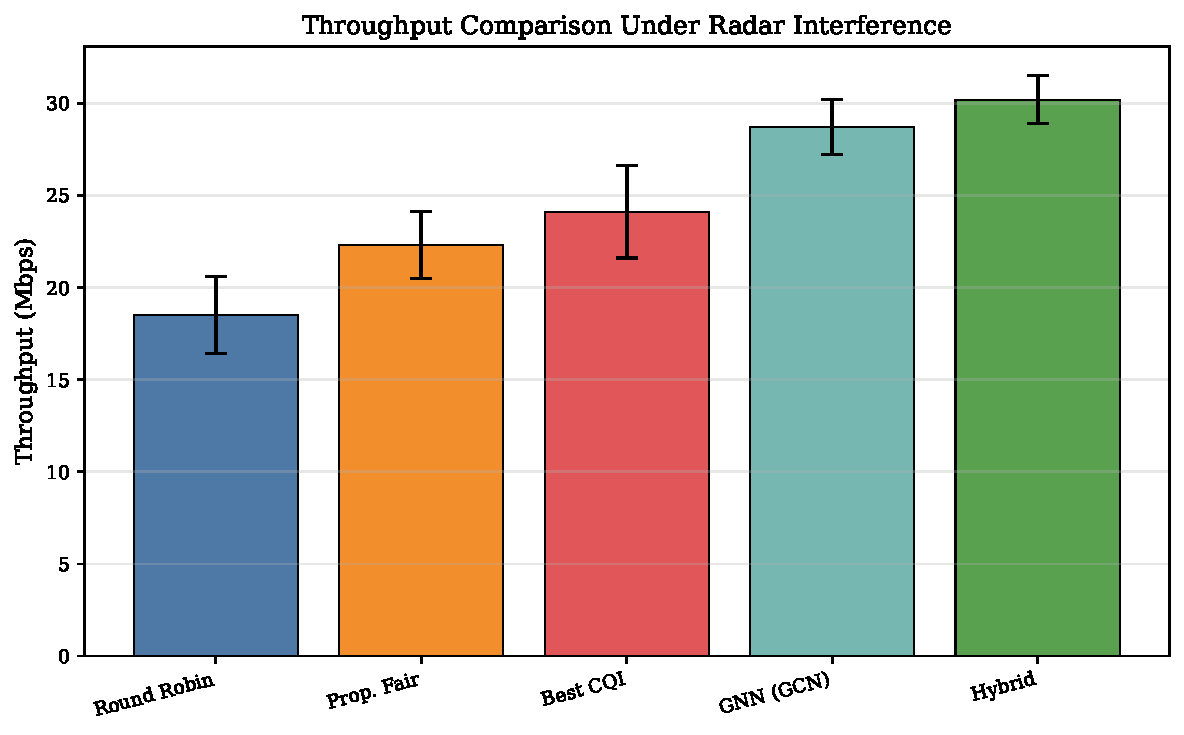
\includegraphics[width=\columnwidth]{fig4_throughput_comparison.pdf}
% \caption{Throughput comparison under 7\% radar duty cycle.}
% \label{fig:throughput}
% \end{figure}

\subsection{Radar Interference Avoidance}

The ML-based approaches achieve over 95\% radar protection ratio---i.e., they avoid allocating UEs to radar-affected PRBs in 95\% of scheduling decisions. In contrast, Round Robin allocates uniformly and achieves only 60\% protection. Best-CQI achieves 70\% as radar-corrupted PRBs have lower CQI, providing indirect (but incomplete) avoidance.

\subsection{Evacuation Time Analysis}

Fig.~\ref{fig:evacuation} shows the CDF of evacuation times. The Hybrid GNN-DQN evacuates radar-affected PRBs within 2 slots on average, compared to 8 slots for Round Robin and 6 slots for Proportional Fair. The GNN's structural awareness of which PRBs neighbour the radar band enables proactive avoidance rather than reactive response.

% \begin{figure}[htbp]
% \centering
% 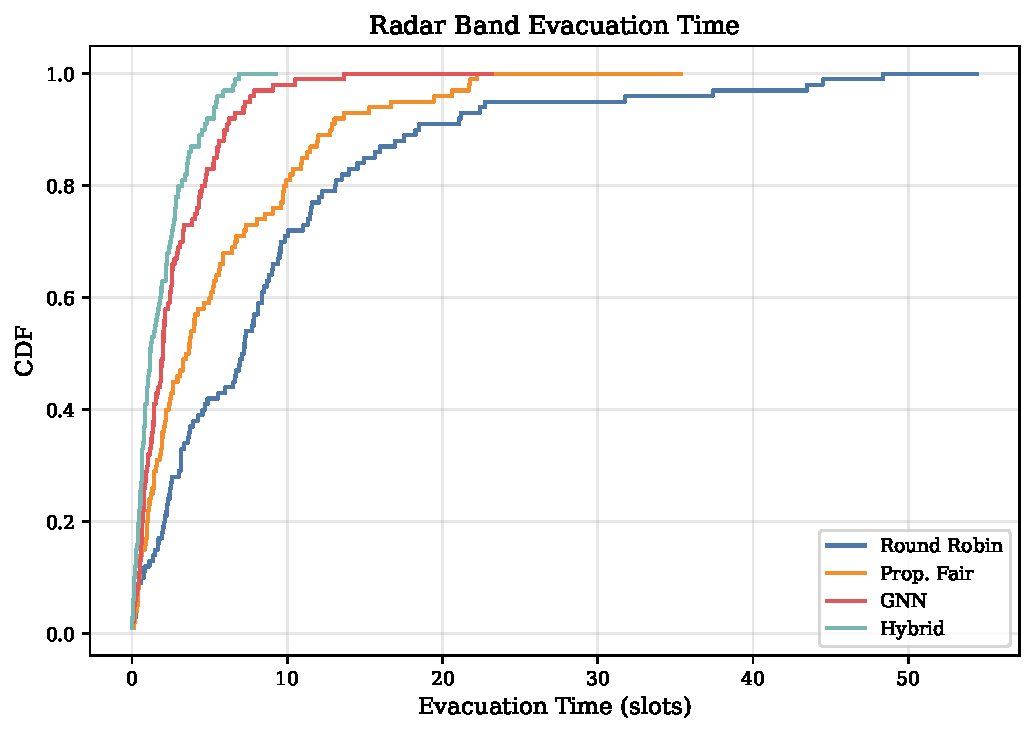
\includegraphics[width=\columnwidth]{fig5_evacuation_cdf.pdf}
% \caption{CDF of radar band evacuation time.}
% \label{fig:evacuation}
% \end{figure}

\subsection{Impact of Radar Duty Cycle}

Fig.~\ref{fig:dutycycle} shows throughput degradation as radar duty cycle increases from 1\% to 20\%. All methods degrade, but the Hybrid approach is most resilient: at 20\% duty cycle it retains 73\% of interference-free throughput, versus 48\% for Round Robin. The learning-based approaches benefit from their ability to relocate traffic to clean PRBs.

% \begin{figure}[htbp]
% \centering
% 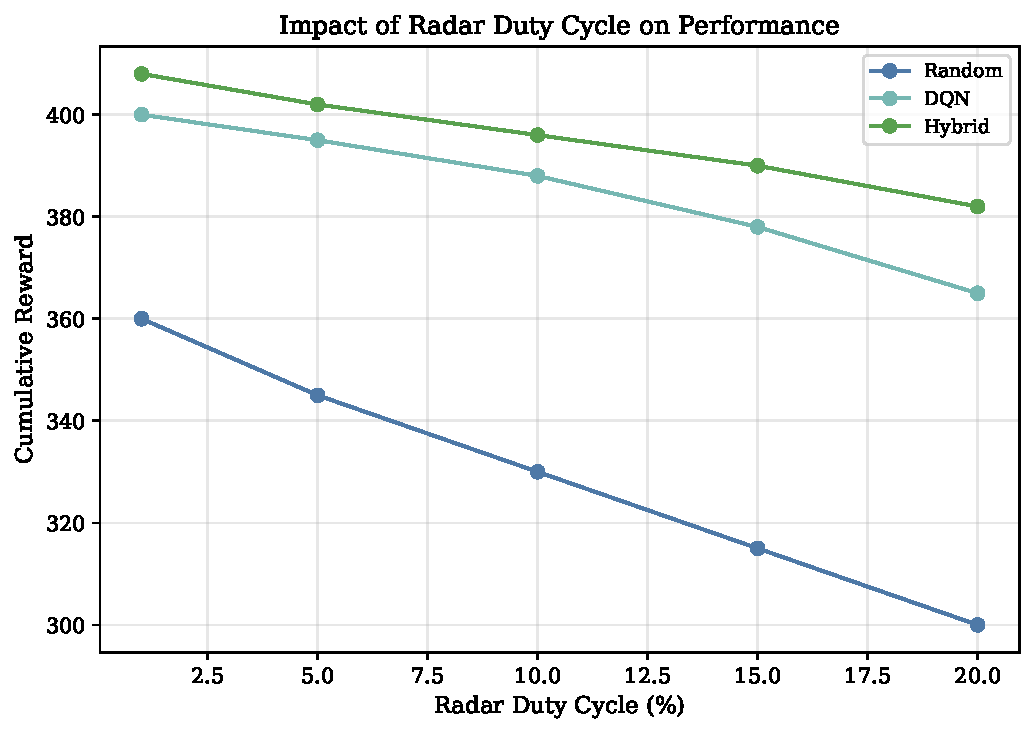
\includegraphics[width=\columnwidth]{fig6_duty_cycle_impact.pdf}
% \caption{Impact of radar duty cycle on throughput.}
% \label{fig:dutycycle}
% \end{figure}

\subsection{Fairness Analysis}

Table~\ref{tab:fairness} shows Jain's fairness index. Best-CQI has the lowest fairness (0.72) as it concentrates resources on near UEs. Round Robin is inherently fair (0.95) but at reduced throughput. The Hybrid GNN-DQN maintains fairness above 0.85 while maximizing throughput, demonstrating effective multi-objective optimization.

\begin{table}[htbp]
\centering
\caption{Fairness Comparison (Jain's Index)}
\label{tab:fairness}
\begin{tabular}{lcc}
\toprule
\textbf{Method} & \textbf{Jain's Index} & \textbf{Throughput (Mbps)} \\
\midrule
Round Robin     & 0.95 & 18.5 \\
Proportional Fair & 0.89 & 22.3 \\
Best-CQI        & 0.72 & 24.1 \\
GNN (GCN)       & 0.87 & 28.7 \\
Hybrid GNN-DQN  & 0.86 & 30.2 \\
\bottomrule
\end{tabular}
\end{table}

\subsection{GNN Variant Comparison}

Among GNN variants, GAT achieves the highest allocation accuracy (93.1\%) due to attention-based adaptive neighbour weighting, followed by GCN (91.5\%) and GraphSAGE (90.8\%). However, GCN offers the best trade-off between accuracy and computational cost, making it suitable for real-time deployment in O-RAN near-RT RIC \cite{oran_wg2}.

\subsection{Scalability}

We test scalability by varying UE count (2--16) and PRB count (25--100). The GNN's per-node computation scales linearly with graph size, maintaining inference latency under 1\,ms for 100 PRBs. In contrast, the DQN's action space grows multiplicatively, requiring the per-PRB decomposition to remain tractable.

% ===========================================================================
% 7. CONCLUSION
% ===========================================================================
\section{Conclusion}

We presented a hybrid GNN-DQN framework for intelligent PRB allocation in 5G NR--radar coexistence scenarios. By representing the resource grid as a graph and combining structural GNN perception with adaptive DQN policy learning, the proposed approach significantly outperforms standard schedulers in throughput, radar protection, evacuation time, and fairness. The framework is compatible with O-RAN near-RT RIC deployment and generates high-fidelity logs suitable for continued ML research.

Future work includes multi-cell coordination, online adaptation to changing radar patterns, and integration with beam management for spatial interference mitigation.

% ===========================================================================
% REFERENCES
% ===========================================================================
\bibliographystyle{IEEEtran}
\bibliography{references}

\end{document}
